\begin{figure}[b]
    \centering
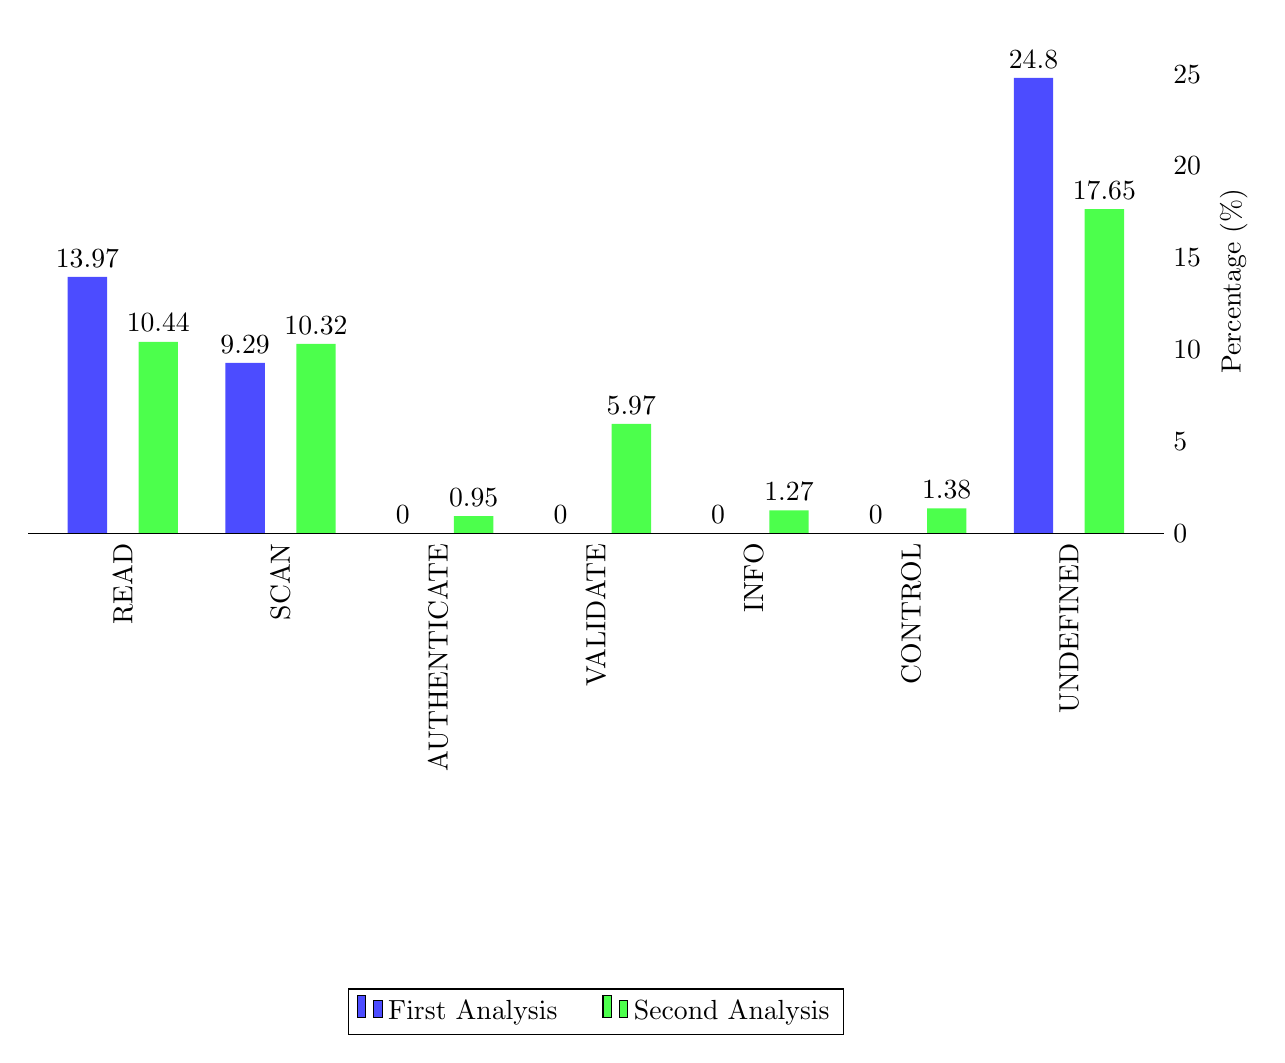
\begin{tikzpicture}
  \begin{axis}[
        ybar,
        axis on top,
        %title={Improvement of the matching},
        height=8cm, width=16cm,
        bar width=0.5cm,
        ybar=0.4cm,
        %ymajorgrids, tick align=inside,
        major grid style={draw=white},
        enlarge y limits={value=.1,upper},
        ymin=0, ymax=25,
        axis x line*=bottom,
        axis y line*=right,
        y axis line style={opacity=0},
        tickwidth=0pt,
        enlarge x limits=true,
        x tick label style={rotate=90},
        legend style={
            at={(0.5,-0.9)},
            anchor=north,
            legend columns=-1,
            /tikz/every even column/.append style={column sep=0.5cm}
        },
        ylabel={Percentage (\%)},
        symbolic x coords={
           READ,
           SCAN,
           AUTHENTICATE,
           VALIDATE,
           INFO,
           CONTROL,
           UNDEFINED
           },
       xtick=data,
       nodes near coords={
        \pgfmathprintnumber[precision=2]{\pgfplotspointmeta}
       }
    ]
    \addplot [draw=none, fill=blue!70] coordinates {
      (READ,13.97)
      (SCAN,9.29)
      (AUTHENTICATE,0) 
      (VALIDATE,0) 
      (INFO,0)
      (CONTROL,0)
      (UNDEFINED,24.80) 
    };
   \addplot [draw=none,fill=green!70] coordinates {
      (READ,10.44)
      (SCAN,10.32)
      (AUTHENTICATE,0.95) 
      (VALIDATE,5.97) 
      (INFO,1.27)
      (CONTROL,1.38)
      (UNDEFINED,17.65) 
      };
%   \addplot [draw=none, fill=green!30] coordinates {
%       (CREATE, 72.7961) 
%       (READ,94.4597)
%       (SCAN,66.6786) 
%      };

    \legend{First Analysis, Second Analysis}
  \end{axis}
  \end{tikzpicture}
    \caption{Caption}
    \label{fig:analysis2:bar_chart}
\end{figure}